%
% A Real Chapter
\chapter{Phased Array Antenna and Optical Ring Resonator: An Overview}

In the last century, radio systems have become an essential way to pass on signals by means of the transmission of electromagnetic waves with frequency below the visible light. In the recent years, increasing demand for fast information exchange motivated the development of many ideas of broadband radio applications. People wish to be able to connect to internet, participate in teleconference, or watch live TV no matter where they are, especially when traveling on a long intercontinental flight. This demand motivated the development of communication between satellite and aeroplanes.

In the application of the radio described above, the system is featured by the radio link with low signal power density. therefore, high-gain and direction-sensitive antennas are essentially required for the signal reception. The ordinary omni-directional antenna is not preferable because, although it is an directional-sensitive antenna, it has low gain \citep{cheng1989field}.

A conventional solution for a direction-sensitive antenna is a dish antenna, which can be steered mechanically to the point its main beam to a desired directions \citep{wilson2013tools}. Even though it is direction-sensitive and has high-gain, a dish antenna is slow because its speed is limited by the mechanical movement. The mechanical movement also have negative effect on the tuning precision. Another drawbacks are its large weight, large size, and aerodynamic drag effect when mounted on top of a plane. It also has difficulty for the maintenance. Instead of using a dish antenna, the more advantageous alternative is to use a \ac{PAA} \cite{balanis2008modern,MeijerinkPhased}. The explanation of \ac{PAA} will be covered in the first section of this chapter.

\section{Phased Array Antenna}
A \ac{PAA} consists of an array of \ac{AE}. The antenna pattern is determined by the geometry of the array as well as the signal amplitude and phase relation between the \ac{AE}s. The main beam of the \ac{PAA} can be steered without any mechanical movement involved. It is possible by changing the amplitude and the phase relation of the \ac{AE} signals. To control both the amplitudes and phases of the AE signals, the so-called beamformer is required. Conventionally a beamformer is realized in
the electrical domain. However, it can also be realized in the optical domain: an photonic beamformer. Compared to its
electrical counterpart, the photonic beamformer has the advantages, such as compactness, light weight, low loss, frequency independence, large instantaneous bandwidth, and inherent immunity to electromagnetic interference \citep{zhuang2010ring}. This fact makes the PAA comprising photonic beam former can be a preferable solution for the communication between satellite and aeroplanes.

The goal of beamformer is that the effective radiation pattern of the array is intensified in a desired direction and suppressed in undesired directions \citep{cheng1989field,balanis2008modern}. Then, the intensification of the radiation pattern in the desired direction results in the main beam of the array. The direction of the main beam can be steered by properly changing the phase relation between the AE signals. The illustration of the changing direction of the main beam is shown on the \figref{fig:beamformer_illustration}:

\begin{figure}[h]
	\centering
	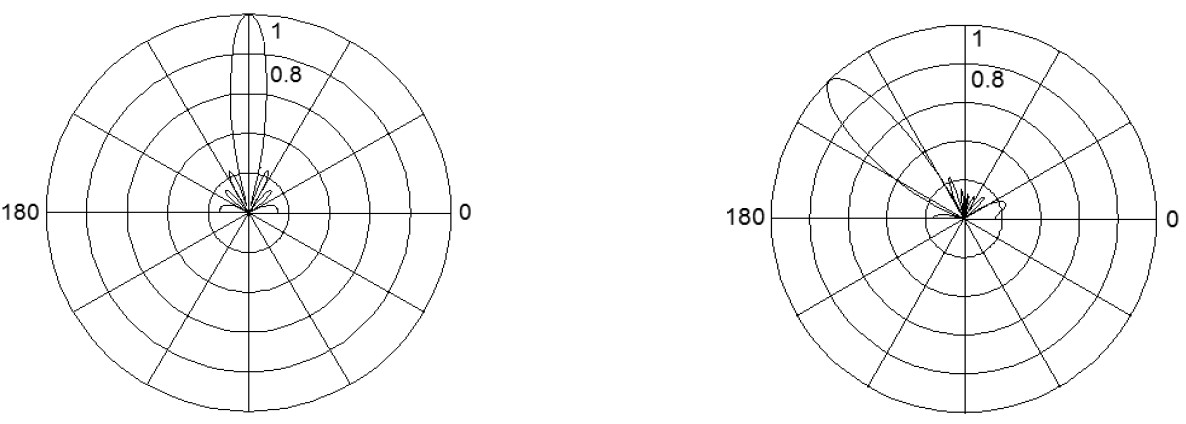
\includegraphics[width=0.8\textwidth]{images/beamformer_illustration}
	\caption{Illustration of (left) the main beam of an effective radiation pattern and (right) the beam steering effect. Source: \citep{zhuang2010ring}}
	\label{fig:beamformer_illustration}
\end{figure}

The simplest PAA is one-dimensional linear array antenna, which is based on gemetry of multiple identical AEs equally spaced along a single line. Although there are various array geometries as explained in \citep{cheng1989field,balanis2008modern}, to understand the basic principle of PAA, the one-dimensional linear array antenna is sufficient. \figref{fig:linear_array_antenna} shows the illustration of a simple 4-element linear array antenna.

\begin{figure}[h]
	\centering
	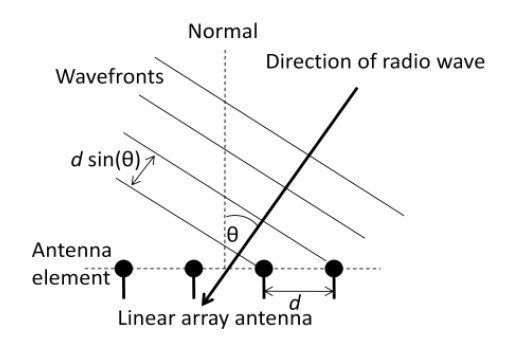
\includegraphics[width=0.5\textwidth]{images/linear_array_antenna}
	\caption{Illustration of a 4-element one-dimensional linear array antenna. Source: \citep{zhuang2010ring}}
	\label{fig:linear_array_antenna}
\end{figure}

Suppose the direction of the radio wave is coming at an angle of $\theta$ with respect to perpendicular direction of the surface of the PAA (called normal direction). Then all the spatial points have the same phase form a wavefront which is perpendicular to propagation direction of the wave, and this wavefront will reach each AE at a different time instance. The formula for the difference of the time arrival of the neighboring AE is given as:

\begin{equation}\label{eq:time_delay}
	\Delta t_a(d,\theta)=\frac{d \sin(\theta)}{c_0}
\end{equation}
where $d$ is the spacing between the AEs and $c_0$ is the speed of light in vacuum. This results in an interelement phase difference:

\begin{equation}\label{eq:phase_diff}
	\Delta \varphi (d,\theta,f)=2\pi f \Delta t_a(d,\theta)
\end{equation}
where $f$ is the frequency of the \ac{RF} wave.

When this interelement phase difference $\Delta \varphi (d,\theta,f)$ is removed by the additional phase compensation between two neighboring AEs $\Delta \delta = -\Delta \varphi (d,\theta,f)$ , the signals from different AEs will be in
phase and can be combined coherently. Then after combining the signals the intensification will be achieved for this particular receiving angle $\theta$. The signals coming from a different angle $\theta '$ will result in $\Delta \varphi (d,\theta ',f)$ which will not be cancelled out by $\Delta \delta$. Then due to the remaining phase difference between the AEs,
suppression of the signal will occur after the signal combining of the array. Furthermore, by adjusting the value of $\Delta \delta$, the receiving direction of the array (main beam) can be steered accordingly \citep{zhuang2010ring}.

Obviously, the application of the PAA in general case will not be as simple as one-dimensional linear array antennas. More complex two-dimensional beam steering is sometimes required for some PAA application. A practical solution of this two-dimensional beam steering is to use a planar array antenna. Basically, it is a rectangular $M\times N$ planar array which can be regarded as $M$ columns of $N$-element linear arrays or $N$ rows of $M$-element linear arrays. More formal analyses of PAAs can be
found in \citep{cheng1989field,balanis2008modern}.

\begin{figure}[h]
	\centering
	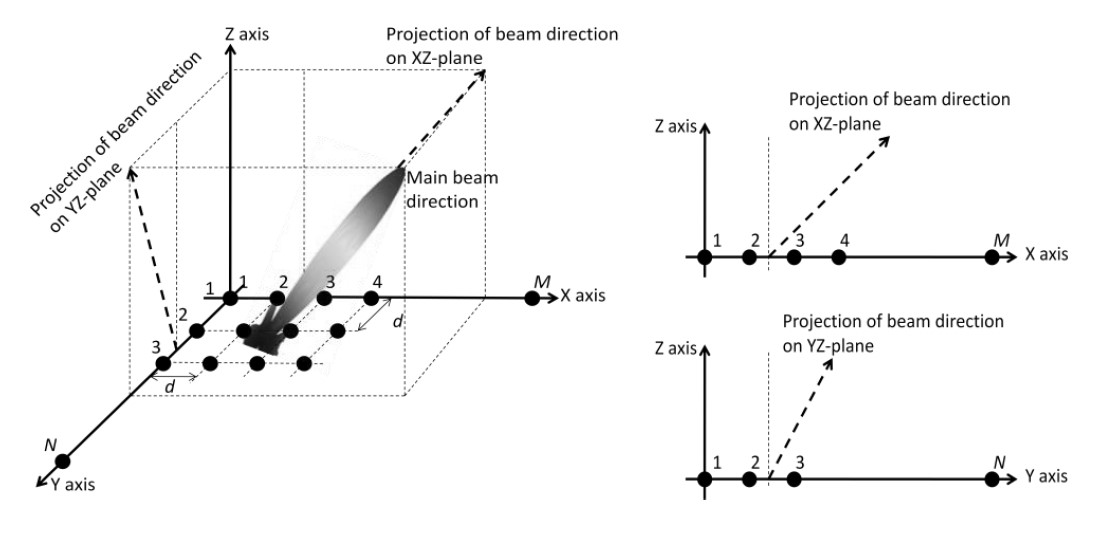
\includegraphics[width=0.9\textwidth]{images/planar_antenna}
	\caption{Schematic of a rectangular $M\times N$ planar array antenna. Source: \citep{zhuang2010ring}}
	\label{fig:planar_antenna}
\end{figure}

\section{Optical Ring Resonator}
The beamformer which will be considered in this thesis is a photonic beamformer system in which the \ac{RF} signals received by the AEs are modulated on optical carriers and tunable
optical delay lines synchronize the signals modulated on the optical carrier. The \ac{ORR} is used to implement the tunable optical delay lines. In this section, the principles of ORR will be covered including the structure, the transfer function and transfer matrix used to derive the frequency response of ORRs, and the delay properties of both single and multiple cascaded ORRs. 

\subsection{Structure of the \ac{ORR}}
A simple one input one output single stage ORR is illustrated on \figref{fig:single_stage_ORR}:

\begin{figure}[h]
	\centering
	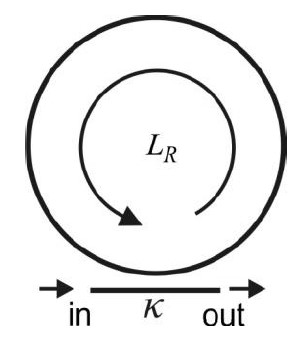
\includegraphics[width=0.2\textwidth]{images/single_stage_ORR}
	\caption{Structure of a $1 \times 1$ single-stage ORR. Source: \citep{zhuang2010ring}}
	\label{fig:single_stage_ORR}
\end{figure}

It consists of a ring-shaped waveguide and a straight waveguide. The waveguide are able to couple light between each other. The parameter $\kappa$ is the power coupling coefficient, which has the value of the range $[0\cdots 1]$, and $L_R$ is the roundtrip length of ring shaped waveguide. Another parameters are $T$ which is the roundtrip period and $\phi$ which is the extra phase-shift due to the heater on the top of the ring. 

\subsection{Mathematical Model of the \ac{ORR}}
The behavior of an optical component can be described by its transfer function (or transfer matrix when a component has multiple input/output ports), which relates the amplitude and phase of the field at input to those at output. \citet{rabus2007integrated} and \citet{zhuang2010ring} have derived the transfer function of which can be summarized as follow.

\subsubsection{Derivation of the ORR Transfer Function}

\begin{figure}[h]
	\centering
	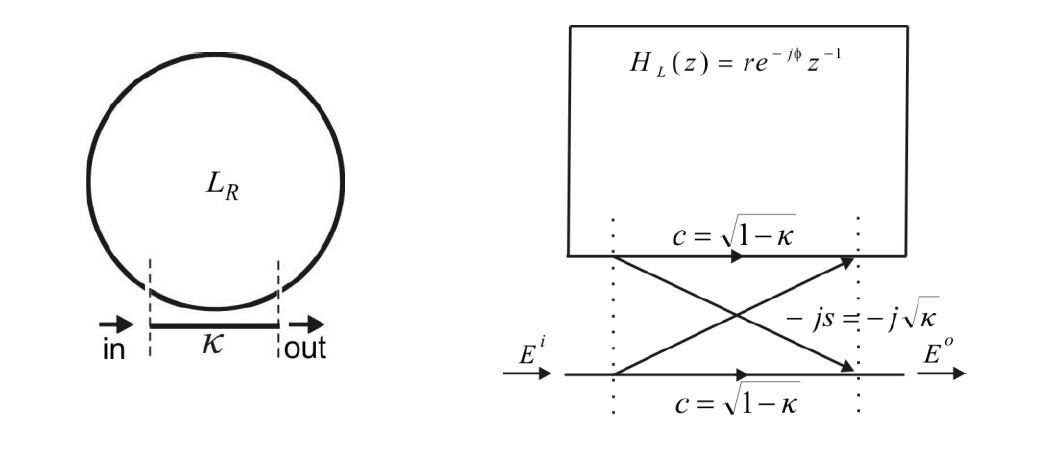
\includegraphics[width=0.8\textwidth]{images/ORR_transferfunction}
	\caption{(left) An ORR formed by a $2 \times 2$ coupler and a feedback waveguide. (right) $Z-$~transform schematic of an ORR. Source: \citep{zhuang2010ring}}
	\label{fig:ORR_transferfunction}
\end{figure}

To derive the transfer function of an ORR, one can first look at the behavior of its two basic building blocks, namely a waveguide feedback path and a $2 \time 2$ coupler, which are shown in \figref{fig:ORR_transferfunction} (left) and the $Z$-transform schematic of an ORR is given in \figref{fig:ORR_transferfunction} (right). Let the signal at the right side of the ring be $E^r$, and the one on the left side be $E^l$, then one can derive the following relations:

\begin{equation}
	\begin{aligned}
	E^r&=-j\sqrt{k}E^i+\sqrt{1-\kappa}E^l\\
	E_l&=rz^{-1}e^{j\phi}E^r \\
	&=E_l=rz^{-1}e^{j\phi}(-j\sqrt{k}E^i+\sqrt{1-\kappa}E^l)\\
	&=\frac{-j\sqrt{k}rz^{-1}e^{-j\phi}E^i}{1-r\sqrt{1-\kappa}z^{-1}e^{-j\phi}}
	\end{aligned}
\end{equation}

\begin{equation}
	\begin{aligned}
	E^o&=\sqrt{1-\kappa}E^i-j\sqrt{\kappa}E^l \\
	&=\frac{\sqrt{1-\kappa}(1-r\sqrt{1-\kappa}z^{-1}e^{-j\phi})E^i-\kappa rz^{-1}e^{-j\phi}E^i}{1-r\sqrt{1-\kappa}z^{-1}e^{-j\phi}}\\
	&=\frac{\sqrt{1-\kappa}-rz^{-1}e^{-j\phi}}{1-r\sqrt{1-\kappa}z^{-1}e^{-j\phi}}E^i
	\end{aligned}
\end{equation}

Substituting $z^{-1}=e^{-2\pi jfT}$ with $T$ the round-trip time of the ring, give the following frequency response:

\begin{equation}
	H(f)=\frac{\sqrt{1-\kappa}-re^{-2\pi jfT-j\phi}}{1-r\sqrt{1-\kappa}e^{-2\pi jfT-j\phi}}
\end{equation}

\subsubsection{Derivation of the ORR Phase Response}



